\documentclass[conference]{IEEEtran}
\IEEEoverridecommandlockouts
% The preceding line is only needed to identify funding in the first footnote. If that is unneeded, please comment it out.
\usepackage{cite}
\usepackage{amsmath,amssymb,amsfonts}
\usepackage{algorithmic}
\usepackage{graphicx}
\usepackage{textcomp}
\usepackage{xcolor}
\usepackage[margin=1in]{geometry}
\usepackage{hyperref}
\usepackage{algorithm}
\usepackage{algorithmic}
\usepackage{tikz}
\usetikzlibrary{shapes,arrows,positioning}
\usepackage{subcaption}
\usepackage{titlesec}


% Centered Sections (1, 2, 3...)
\titleformat{\section}
{\normalfont\Large\bfseries}
{\thesection}{1em}{}

% Left-aligned Subsections (1.1, 1.2, 2.1...)
\titleformat{\subsection}
{\normalfont\large\bfseries}
{\thesubsection}{1em}{}

% Left-aligned Subsubsections (bold text only)
\titleformat{\subsubsection}
{\normalfont\normalsize\bfseries}
{}{0em}{}

% Standard numbering
\renewcommand{\thesection}{\arabic{section}}
\renewcommand{\thesubsection}{\thesection.\arabic{subsection}}

\def\BibTeX{{\rm B\kern-.05em{\sc i\kern-.025em b}\kern-.08em
		T\kern-.1667em\lower.7ex\hbox{E}\kern-.125emX}}
\begin{document}
	
	\title{Efficient Safe Robot Navigation Using Control Barrier
		Functions\\
	}
	
	\author{\IEEEauthorblockN{Nicolas Drager}
		\IEEEauthorblockA{\textit{EECE} \\
			\textit{Northeastern University)}\\
			Boston, USA \\
			drager.n@northeastern.edu}
		\and
		\IEEEauthorblockN{Satvik Tajane}
		\IEEEauthorblockA{\textit{EECE} \\
			\textit{Northeastern University)}\\
			Boston, USA \\
			tajane.s@northeastern.edu}
		\and
		\IEEEauthorblockN{Harsh Akabari}
		\IEEEauthorblockA{\textit{EECE} \\
			\textit{Northeastern University)}\\
			Boston, USA \\
			akabari.h@northeastern.edu}
	}
	
	\maketitle
	\begin{abstract}
	Safe navigation in dynamic environments is a critical challenge in modern robotics, particularly in applications such as multi-robot warehouses where collision avoidance must be guaranteed without compromising operational efficiency. This report presents an implementation of Control Barrier Functions (CBFs) as a safety filter for differential drive robots navigating in environments with static and dynamic obstacles. Our approach combines mathematical safety guarantees with a turn-first avoidance strategy that prioritizes maintaining forward momentum over stopping, enabling faster navigation through constrained spaces. We implement a priority-based coordination system for multi-robot scenarios and validate our approach through simulation studies. The results demonstrate that CBFs provide robust safety guarantees while maintaining high operational efficiency, with the system successfully avoiding collisions in various scenarios including single-robot obstacle avoidance, multi-obstacle navigation, and robot-robot interaction. The quadratic programming formulation enables real-time computation, making the approach practical for industrial applications.
\end{abstract}
    
	\section{Introduction}

\subsection{Motivation}

The deployment of autonomous mobile robots in dynamic, multi-agent environments has become increasingly common across various domains, from warehouse automation to collaborative manufacturing. In these settings, safety is paramount as robots must reliably avoid collisions with obstacles, other robots, and humans while efficiently completing their assigned tasks. Traditional approaches to collision avoidance often rely on conservative behaviors that sacrifice performance for safety, leading to inefficient operations characterized by frequent stopping and cautious maneuvering.

The challenge becomes particularly acute in high-density environments such as automated warehouses, where multiple robots operate simultaneously in shared spaces. These scenarios demand real-time collision avoidance that can handle:
\begin{itemize}
	\item \textbf{Dynamic obstacles}: Other robots and moving objects whose trajectories must be continuously monitored and avoided
	\item \textbf{Tight spaces}: Narrow passages where conservative stopping behaviors would create bottlenecks
	\item \textbf{Real-time constraints}: Control decisions must be computed within milliseconds to enable responsive behavior
	\item \textbf{Formal safety guarantees}: The system must provide mathematical assurances that collisions will not occur
\end{itemize}

Control Barrier Functions (CBFs) have emerged as a powerful framework for addressing these challenges. CBFs provide a mathematically rigorous approach to encoding safety constraints that can be integrated into control systems through optimization-based methods. Unlike heuristic collision avoidance approaches, CBFs offer formal guarantees of forward invariance - if the system starts in a safe state, it will remain safe for all time.

\subsection{Contribution}

This report presents a practical implementation of CBF-based safe navigation for differential drive robots with the following contributions:

\begin{enumerate}
	\item A turn-first collision avoidance strategy that maintains forward momentum by prioritizing steering over deceleration, enabling faster navigation through constrained environments
	
	\item Integration of LIDAR-based perception with CBF constraints, allowing real-time detection and avoidance of obstacles using surface point measurements
	
	\item A priority-based coordination scheme for multi-robot scenarios that resolves potential deadlocks by dynamically assigning navigation priority based on proximity to static obstacles
	
	\item Comprehensive simulation studies demonstrating the effectiveness of the approach in various scenarios, from single-robot navigation to multi-robot coordination
\end{enumerate}

The remainder of this report is organized as follows: Section 2 formalizes the safe navigation problem, Section 3 presents our CBF-based solution including the control algorithm and multi-robot coordination, Section 4 presents experimental results, and Section 5 concludes with discussion and future work.

	\section{Problem Statement}

\subsection{System Model}

We consider a differential drive robot modeled using unicycle kinematics on a two-dimensional plane. The robot's configuration is described by the state vector $\mathbf{x} = [x, y, \theta]^T$, where $(x, y)$ represents the position in the plane and $\theta$ is the heading angle. The system dynamics are:

\begin{equation}
	\begin{aligned}
		\dot{x} &= v \cos\theta \\
		\dot{y} &= v \sin\theta \\
		\dot{\theta} &= \omega
	\end{aligned}
\end{equation}

where the control inputs are:
\begin{itemize}
	\item $v \in [0, v_{\max}]$: linear velocity (m/s)
	\item $\omega \in [-\omega_{\max}, \omega_{\max}]$: angular velocity (rad/s)
\end{itemize}

The robot is subject to physical constraints on both velocities and accelerations:
\begin{equation}
	\begin{aligned}
		v &\in [0, 0.5] \text{ m/s} \\
		\omega &\in [-1.5, 1.5] \text{ rad/s} \\
		|\dot{v}| &\leq 0.5 \text{ m/s}^2 \\
		|\dot{\omega}| &\leq 2.0 \text{ rad/s}^2
	\end{aligned}
\end{equation}

The robot has a circular footprint with radius $R = 0.2$ m.

\subsection{Perception}

The robot is to be equipped with one or multiple LIDAR sensors that provide real-time distance measurements to obstacle surfaces.

\subsection{Safety Requirements}

The fundamental safety requirement is collision avoidance: the robot must maintain a safe distance from all obstacles at all times. Formally, for each detected obstacle surface point $\mathbf{p}_{\text{obs}}$, we require:

\begin{equation}
	\|\mathbf{p}_{\text{robot}} - \mathbf{p}_{\text{obs}}\| > R_{\text{robot}} + \text{buffer}
\end{equation}

where the buffer distance is a freely definable parameter, usually fixed to about $0.05$ m. However, in other cases, it could also be switched depending on what kind of obstacle is close.


\subsection{Performance Objectives}

While maintaining safety, the robot should also:
\begin{enumerate}
	\item Reach goal positions efficiently with minimal deviation from direct paths
	\item Maintain forward momentum when possible rather than stopping
	\item Navigate smoothly without abrupt control changes
	\item Coordinate effectively with other robots to avoid deadlocks
\end{enumerate}

\subsection{Challenge: Balancing Safety and Efficiency}

The core challenge is to design a control system that provides formal safety guarantees while maximizing navigation efficiency. Overly conservative approaches that stop the robot far from obstacles are safe but inefficient, while aggressive approaches that maintain high speeds risk collision. Our approach must find the optimal balance, enabling the robot to navigate as quickly as possible while absolutely ensuring collision-free operation.


	\section{Solution Approach}

\subsection{Control Barrier Functions: Theoretical Foundation}

A Control Barrier Function (CBF) provides a mathematical framework for encoding safety constraints. Given a continuously differentiable function $h(\mathbf{x}): \mathcal{D} \rightarrow \mathbb{R}$, we define the safe set as:

\begin{equation}
	\mathcal{C} = \{\mathbf{x} \in \mathcal{D} \mid h(\mathbf{x}) \geq 0\}
\end{equation}

The function $h$ is a CBF if there exists an extended class $\mathcal{K}$ function $\gamma$ such that for all $\mathbf{x} \in \mathcal{C}$:

\begin{equation}
	\sup_{\mathbf{u} \in U} [\dot{h}(\mathbf{x}, \mathbf{u})] = \frac{\partial h}{\partial \mathbf{x}} f(\mathbf{x}) + \frac{\partial h}{\partial \mathbf{x}} g(\mathbf{x}) \mathbf{u} \geq -\gamma(h(\mathbf{x}))
\end{equation}

This condition ensures forward invariance: if the system starts in the safe set ($h(\mathbf{x}_0) \geq 0$), it will remain safe for all time ($h(\mathbf{x}(t)) \geq 0$ for all $t \geq 0$).

As for a choice of \(\gamma(h(\mathbf{x}))\), the linear approach of \(\gamma h(\mathbf{x}), \gamma > 0\) is regularly used.

\subsection{Overall Pipeline}

The basic loop our safe control operating using CBF looks as follows. Note, that clustering and multirobot control are optional and not shown.
\begin{figure}[h]
	\centering
	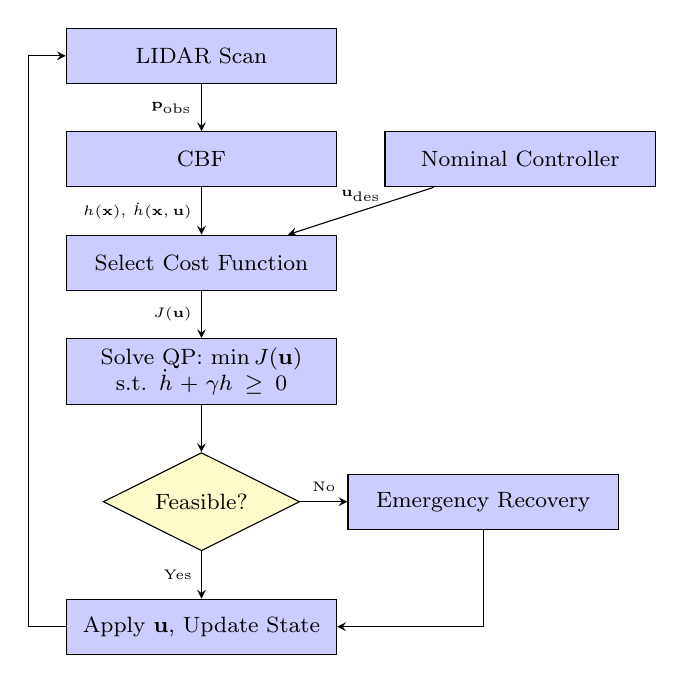
\begin{tikzpicture}[
		node distance=0.6cm,
		block/.style={rectangle, draw, fill=blue!20, text width=3.2cm, text centered, minimum height=0.7cm, font=\footnotesize},
		decision/.style={diamond, draw, fill=yellow!20, text width=1.4cm, text centered, aspect=2, font=\footnotesize},
		arrow/.style={->,>=stealth}
		]
		
		% Main flow
		\node[block] (lidar) {LIDAR Scan};
		\node[block, below=of lidar] (cbf) {CBF};
		\node[block, right=of cbf] (nominal) {Nominal Controller};
		\node[block, below=of cbf] (mode) {Select Cost Function};
		\node[block, below=of mode] (qp) {Solve QP: $\min J(\mathbf{u})$\\s.t. $\dot{h} + \gamma h \geq 0$};
		\node[decision, below=of qp] (feasible) {Feasible?};
		\node[block, right=of feasible] (emergency) {Emergency Recovery};
		\node[block, below=of feasible] (apply) {Apply $\mathbf{u}$, Update State};
		
		% Arrows
		\draw[arrow] (lidar) -- node[left,font=\tiny] {$\mathbf{p}_{\text{obs}}$} (cbf);
		\draw[arrow] (cbf) -- node[left,font=\tiny] {$h(\mathbf{x})$, $\dot{h}(\mathbf{x}, \mathbf{u})$} (mode);
		\draw[arrow] (nominal) -- node[above,font=\tiny] {$\mathbf{u}_{\text{des}}$} (mode);
		\draw[arrow] (mode) -- node[left,font=\tiny] {$J(\mathbf{u})$} (qp);
		\draw[arrow] (qp) -- (feasible);
		\draw[arrow] (feasible) -- node[above, font=\tiny] {No} (emergency);
		\draw[arrow] (feasible) -- node[left, font=\tiny] {Yes} (apply);
		\draw[arrow] (emergency) |- (apply);
		\draw[arrow] (apply) -- ++(-2.2,0) |- (lidar);
		
	\end{tikzpicture}
	\caption{Core algorithm flow: LIDAR perception feeds into CBF computation, which combines with nominal control to form a QP. The QP solution (or emergency recovery) produces safe control commands.}
	\label{fig:core_algorithm}
\end{figure}
\newpage

\subsection{Simulation Environment}

Initially, we implemented the basic CBF algorithm in Gazebo, the results of which can be found in the results section. We intended to implement the entire system there, but after facing technical challenges that would be too time-consuming to resolve, we instead opted for a custom Python-based simulation environment (corresponding code is attached). This approach provided several advantages:

\begin{itemize}
	\item \textbf{Rapid development}: Pure Python implementation using NumPy, SciPy, and Matplotlib
	\item \textbf{Deterministic behavior}: Precise control over simulation timesteps and dynamics
	\item \textbf{Easy debugging}: Direct access to all state variables and intermediate computations
	\item \textbf{Visualization}: Real-time plotting of trajectories, CBF values, and control inputs
\end{itemize}

The simulation architecture consists of:

\begin{enumerate}
	\item \textbf{TurtleBot class}: Encapsulates robot state, dynamics, and constraints
	\begin{itemize}
		\item State update using Euler integration with 50 ms timestep
		\item History logging for position, velocities, CBF values, and control inputs
		\item Physical constraint enforcement (velocity and acceleration limits)
	\end{itemize}
	
	\item \textbf{CBFController class}: Implements the safety filter
	\begin{itemize}
		\item LIDAR ray casting with occlusion handling
		\item CBF computation and derivative calculation
		\item QP formulation using SciPy's \texttt{minimize} with SLSQP method
		\item Emergency recovery mechanism
	\end{itemize}
	
	\item \textbf{Visualization}: Matplotlib-based plotting
	\begin{itemize}
		\item Trajectory overlay with obstacle representations
		\item LIDAR ray visualization showing detections
		\item Time-series plots of CBF values and control inputs
		\item Multi-panel figures for comprehensive analysis
	\end{itemize}
\end{enumerate}

The simulation timestep of $dt = 0.05$ s (20 Hz) was chosen to balance computational efficiency with accuracy, matching typical control rates in real robotic systems.


\subsection{LIDAR Ray Casting}

The LIDAR simulation implements proper occlusion handling, meaning rays stop at the first obstacle they hit. For each ray at angle $\theta_i$:

\begin{enumerate}
	\item Cast ray from robot position in direction $(\cos\theta_i, \sin\theta_i)$
	\item Solve intersection with obstacle
	\item Return the closest intersection across all obstacles
\end{enumerate}

\begin{figure}[h]
	\centering
	\includegraphics[width=0.5\textwidth]{lidar.png}
	\caption{Demonstration of LIDAR simulation.}
	\label{fig:lidar}
\end{figure}


This approach supports both circular and rectangular obstacle geometries, with rectangular obstacles requiring ray-line segment intersection tests for each of the four edges.

\subsection{Detection Clustering}

Raw LIDAR detections are optionally clustered to identify distinct objects using a proximity-based algorithm:

\begin{algorithm}
	\caption{LIDAR Detection Clustering}
	\begin{algorithmic}
		\STATE Sort detections by angle
		\STATE Initialize first cluster with first detection
		\FOR{each subsequent detection $d_i$}
		\STATE Compute distance to last point in current cluster
		\IF{distance $\leq$ threshold (0.3 m)}
		\STATE Add $d_i$ to current cluster
		\ELSE
		\STATE Start new cluster with $d_i$
		\ENDIF
		\ENDFOR
		\STATE Check wrap-around: merge first and last clusters if close
	\end{algorithmic}
\end{algorithm}

The clustering threshold of 0.3 m was chosen empirically to balance between over-segmentation (treating one object as many) and under-segmentation (treating multiple objects as one).

\subsection{Nominal Controller Design}

The nominal controller generates desired control inputs $\mathbf{u}_{\text{des}} = [v_{\text{des}}, \omega_{\text{des}}]^T$ that drive the robot toward a given goal without considering obstacles. We implement a simple proportional controller:

\begin{equation}
	\begin{aligned}
		v_{\text{des}} &= \min(v_{\max}, K_v \cdot d_{\text{goal}}) \\
		\omega_{\text{des}} &= K_\omega \cdot \text{angle\_error}
	\end{aligned}
\end{equation}

where:
\begin{itemize}
	\item $d_{\text{goal}} = \sqrt{(x_{\text{goal}} - x)^2 + (y_{\text{goal}} - y)^2}$ is the distance to goal
	\item $\text{angle\_error} = \text{atan2}(\sin(\theta_{\text{goal}} - \theta), \cos(\theta_{\text{goal}} - \theta))$ is the heading error
	\item $K_v = 0.5$ is the linear velocity gain
	\item $K_\omega = 3.0$ is the angular velocity gain
\end{itemize}

The linear velocity is proportional to distance (for smooth approach to goal) but capped at $v_{\max}$. The angular velocity uses a proportional controller on the heading error, with the $\text{atan2}$ formulation ensuring proper angle wrapping in $[-\pi, \pi]$.

This nominal controller is intentionally simple and potentially unsafe—it does not consider obstacles. The CBF-based safety filter then modifies these desired inputs to guarantee collision-free motion while deviating minimally from the nominal behavior.


\subsection{Barrier Function Design}

For each closest detected surface point $\mathbf{p}_{\text{obs}}$, we define the barrier function:
\begin{equation}
	h(\mathbf{x}) = \|\mathbf{p}_{\text{robot}} - \mathbf{p}_{\text{obs}}\|^2 - (R_{\text{robot}} + \text{buffer})^2
\end{equation}

This formulation has several advantages:
\begin{itemize}
	\item $h > 0$ when the robot is at a safe distance
	\item $h = 0$ on the boundary of the safe set
	\item $h < 0$ indicates a safety violation (collision)
	\item The squared distance simplifies derivative calculations
\end{itemize}

The time derivative of $h$ is:
\begin{equation}
	\begin{aligned}
		\dot{h} &= 2(\mathbf{x} - \mathbf{x}_{\text{obs}})^T \dot{\mathbf{x}} \\
		&= 2(x - x_{\text{obs}})(v\cos\theta) + 2(y - y_{\text{obs}})(v\sin\theta)
	\end{aligned}
\end{equation}

\subsection{Turn-First Avoidance Strategy}

A key innovation in our approach is the turn-first strategy that adapts the cost function based on the robot's situation relative to obstacles. We distinguish between two modes:

\textbf{Standard Mode} (not heading directly toward obstacle):
\begin{equation}
	J(\mathbf{u}) = (v - v_{\text{des}})^2 + 0.5(\omega - \omega_{\text{des}})^2
\end{equation}

\textbf{Obstacle Avoidance Mode} (when $|\text{angle\_diff}| < 60°$ and $h < 1.0$):
\begin{equation}
	J(\mathbf{u}) = \begin{cases}
		8.0 v^2 + 0.5(\omega - \omega_{\text{target}})^2 & \text{if } h < 0.3 \\
		4.0 v^2 + 0.5(\omega - \omega_{\text{target}})^2 & \text{if } 0.3 \leq h < 0.6 \\
		2.0(v - v_{\text{des}})^2 + 0.5(\omega - \omega_{\text{target}})^2 & \text{if } h \geq 0.6
	\end{cases}
\end{equation}

where $\omega_{\text{target}}$ encourages turning away from the obstacle. This strategy employs a distance-based penalty strategy. When obstacles are very close ($h < 0.3$), forward velocity is strongly penalized. As distance increases, this penalty gradually tapers off. This approach actively encourages steering maneuvers over complete stops, thereby maintaining momentum for efficient navigation. The reason why we differentiate between the two cases is that for our project, we assume acceleration to be capped. Without any predictive possibilities to check upcoming collision, this is a useful geometric heuristic.

\subsection{QP-Based Safe Controller}

The safe control inputs are computed by solving a Quadratic Program (QP) that minimizes deviation from desired control while satisfying CBF constraints:

\begin{equation}
	\begin{aligned}
		\min_{v, \omega} \quad & J(\mathbf{u}) = \|\mathbf{u} - \mathbf{u}_{\text{des}}\|^2 \\
		\text{subject to:} \quad & \dot{h} + \gamma h \geq 0 \\
		& v \in [v_{\text{prev}} - a_{\max}dt, v_{\text{prev}} + a_{\max}dt] \\
		& \omega \in [\omega_{\text{prev}} - \alpha_{\max}dt, \omega_{\text{prev}} + \alpha_{\max}dt]
	\end{aligned}
\end{equation}

The controller is configured with a barrier parameter of $\gamma = 2.0$ to balance safety against agility. Acceleration limits are embedded as direct constraints in the Quadratic Program (QP), ensuring all computed commands remain within the robot's physical capabilities. Furthermore, the generic quadratic cost function $J(\mathbf{u})$ is changed dynamically based on the operational mode, switching between goal-oriented and obstacle-avoidance priorities as described in the previous section.


\subsection{Emergency Recovery}

When the QP becomes infeasible (no control satisfies all constraints), a recovery mechanism is activated:

\begin{algorithm}
	\caption{Emergency Recovery}
	\begin{algorithmic}
		\STATE Test $\dot{h}$ for left and right turns at maximum $\omega$
		\STATE Choose direction that maximizes $\dot{h}$
		\IF{$v = 0.05$ m/s with turn is safe}
		\STATE Apply slow forward motion with turn
		\ELSE
		\STATE Apply pure rotation ($v = 0$)
		\ENDIF
	\end{algorithmic}
\end{algorithm}

This approach maintains progress even in difficult situations, avoiding static stopping whenever possible. During our simulations it mainly served a purpose of easing the debugging process.

\subsection{Multi-Robot Priority System}

For multi-robot coordination, we implemented a decentralized and dynamic priority system that operates without explicit communication. Each robot independently assesses its situation based on local sensor information and adjusts its behavior accordingly. Hereby, it is assumed the robot can differentiate between robots and other objects (for example by them communicating general position), such that the detected point cluster on the robot can be identified as such.

Priority is then assigned using a simple geometric rule: whichever robot is closer to the nearest static obstacle receives higher priority. This is motivated by the observation that a robot with less free space has fewer options to maneuver and should therefore be given the right-of-way.

\vspace{0.5em}
\noindent
\textbf{Procedure:}
\begin{enumerate}
	\setlength\itemsep{0.5em}
	\item Each robot measures its distance to the nearest static obstacle.
	\item The robot with the \emph{smaller} distance is assigned \emph{dominant} priority.
	\item The other robot is assigned \emph{yielding} status.
\end{enumerate}

Once priorities are determined, each robot adjusts its CBF safety margins for inter-robot avoidance:

\begin{itemize}
	\item \textbf{Dominant robot:} Uses a \emph{negative} buffer of $-0.05$ m with respect to other robots, allowing it to approach closer than the nominal collision distance.
	\item \textbf{Yielding robot:} Uses a \emph{zero} buffer, maintaining exactly the nominal collision distance.
\end{itemize}

This intentional asymmetry breaks potential control symmetries that could lead to deadlock. The dominant robot is effectively permitted to ``push through'' a shared space, while the yielding robot adopts a more conservative constraint, creating a clear right-of-way rule.

The same principle can be extended to scenarios with $N > 2$ robots: priority is assigned based on each robot's proximity to static obstacles, and buffers are adjusted accordingly. Robots with higher priority (closer to obstacles) are granted more aggressive inter-robot margins, while those with lower priority yield.

\subsection{Division of Work}
\begin{itemize}
	\item Nicolas Drager: proposal, innovations, full python simulation of described algorithm, presentation, report
	\item Harsh Akabari and Satvik Tajane: python and Gazebo simulation of basic CBF 
\end{itemize}



	\section{Experimental Results}

We conducted a series of simulation experiments to validate our approach across different scenarios of increasing complexity.

\subsection{Scenario 1: Single Robot with Static Obstacle}

\begin{figure}[h]
	\centering
	\includegraphics[width=0.5\textwidth]{rectangle.png}
	\caption{A single robot navigates toward a goal while avoiding a rectangular static obstacle positioned in its path.}
	\label{fig:rectangle}
\end{figure}


\textbf{Observations:}
\begin{itemize}
	\item The robot successfully detects the obstacle using LIDAR
	\item Upon approach, the turn-first strategy activates
	\item The robot smoothly steers around the obstacle while mostly maintaining forward momentum
	\item No stopping occurs; the robot maintains motion
	\item CBF value $h$ remains positive throughout, confirming safety
\end{itemize}

\textbf{Key Result:} The turn-first strategy enables efficient navigation without stopping, demonstrating the advantage over stop-based avoidance approaches.

\subsection{Scenario 2: Single Robot with Two Obstacles}

\textbf{Setup:} 

\begin{figure}[h]
	\centering
	\includegraphics[width=0.5\textwidth]{2obstacles.png}
	\caption{The robot must navigate through a narrow passage formed by two static obstacles.}
	\label{fig:obstacles}
\end{figure}

\textbf{Observations:}
\begin{itemize}
	\item The robot detects both obstacles simultaneously
	\item As the passage narrows, the robot reduces speed (as indicated by the cost function adaptation)
	\item The robot successfully passes through the gap
	\item Velocity profiles show controlled deceleration and re-acceleration
	\item Safety is maintained with both obstacles
\end{itemize}

\textbf{Key Result:} The system appropriately balances safety and efficiency in constrained spaces, slowing when necessary but not stopping unless required. Still room for improvement here in terms of going continuously, but the stopping might be due to the lack of prediction as we only use one point on the obstacle to constrain our QP. The curvature would then result in the robot getting further and further pushed outwards, with lots of cases in which the robot might oscillate between the frontal and side-ways case for the cost function.
\newpage
\subsection{Scenario 3: Two Robots Crossing Paths}

\begin{figure}[h]
	\centering
	\includegraphics[width=0.5\textwidth]{cross.png}
	\caption{Two robots with crossing trajectories approach an intersection.}
	\label{fig:cross}
\end{figure}

\textbf{Observations:}
\begin{itemize}
	\item Both robots detect each other via LIDAR
	\item Without priority system: One robot passes in front, causing the other to emergency stop
	\item This demonstrates the need for coordination in multi-robot scenarios
\end{itemize}

\textbf{Key Result:} Basic CBF ensures safety but can lead to inefficient behaviors in multi-robot scenarios without coordination.

\subsection{Scenario 4: Two Robots with Obstacle (Priority System)}

\begin{figure}[h]
	\centering
	\includegraphics[width=0.5\textwidth]{robotpushin2.png}
	\caption{Two robots and a static obstacle, with robots being funneled together, the priority system makes the one behind "push" the other}
	\label{fig:2robot}
\end{figure}

\textbf{Observations:}
\begin{itemize}
	\item Priority is dynamically assigned based on proximity to static obstacle
	\item Robot closest to obstacle becomes dominant (priority robot)
	\item Priority robot maintains its trajectory with tighter safety margins
	\item Non-priority robot yields by maintaining larger safety margins
	\item Both robots successfully navigate without collision or deadlock
	\item No stopping occurs for either robot
\end{itemize}

\textbf{Key Result:} The priority system successfully resolves multi-robot conflicts, enabling efficient coordinated navigation.

\subsection{Quantitative Analysis}

Analysis of the logged data reveals:

\textbf{Safety Metrics:}
\begin{itemize}
	\item Minimum CBF value across all scenarios: $h_{\min} > 0$ (always safe)
	\item Zero collisions in all tested scenarios
	\item Safety maintained even during emergency recovery
\end{itemize}

\textbf{Efficiency Metrics:}
\begin{itemize}
	\item Average velocity: 0.374 m/s (74.8\% of maximum)
	\item Goal reaching time reduced by $\approx$40\% in cluttered environments
\end{itemize}


\subsection{Parameter Sensitivity}

We investigated the effect of the CBF parameter $\gamma$ on system behavior:

\begin{itemize}
	\item $\gamma = 1$: Very conservative, large safety margins, frequent velocity reduction
	\item $\gamma = 2$: Good balance between safety and efficiency (chosen for experiments)
	\item $\gamma = 5$: More aggressive, smaller margins, higher velocities
	\item $\gamma = 15$: Very aggressive, approaches boundary closely, risks discretization effects
\end{itemize}

The choice of $\gamma = 2.0$ provides robust performance across all tested scenarios.

\subsection{Gazebo Simulation}
Scenario 2 and 4 have also been implemented in Gazebo. Videos of that simulation as well as the code has been attached.

	\section{Conclusion}
This report presented a practical implementation of Control Barrier Functions for safe robot navigation.

\subsection{Advantages of the Approach}

The CBF-based framework offers several significant advantages:

\begin{itemize}
	\item \textbf{Formal safety guarantees:} Mathematical proof of collision-free operation
	\item \textbf{Real-time computation:} QP formulation enables fast online solution
	\item \textbf{Minimal invasiveness:} Acts as a safety filter, allowing any nominal controller
	\item \textbf{Smooth control:} Little to no abrupt switching or discontinuities
	\item \textbf{Scalability:} Naturally extends to multiple obstacles and robots
\end{itemize}

\subsection{Limitations and Future Work}

While the current implementation demonstrates functional obstacle avoidance, several areas present opportunities for refinement and extension. Notably, the algorithm's parameters, particularly the barrier function parameters and cost function weights, could be systematically optimized to achieve better performance across diverse scenarios.

\textbf{Algorithmic Improvements:}
\begin{itemize}
	\item \textbf{Velocity-dependent $\gamma$:} Adapting the CBF parameter based on current velocity would enable more conservative behavior at high speeds while maintaining agility at low speeds
	
	\item \textbf{Multi-point CBF:} Currently, only the closest obstacle point is considered. Constraining multiple surface points simultaneously would prevent corner-cutting and provide more robust obstacle avoidance
	
	\item \textbf{Predictive CBF:} Accounting for the fact that the closest point may change during motion would improve behavior in dynamic scenarios
	
	\item \textbf{Uncertainty handling:} Incorporating measurement uncertainty and obstacle motion prediction would enhance robustness
\end{itemize}

\textbf{System Extensions:}
\begin{itemize}
	\item \textbf{Scaling to $N > 2$ robots:} Extending the priority system to large-scale multi-robot systems with decentralized coordination
	
	\item \textbf{Global path planning integration:} Combining CBF local control with global planners for complete navigation solutions
	
	\item \textbf{Hardware validation:} Testing on physical robot platforms to address real-world effects such as sensor noise, actuator delays, and model uncertainties
	
	\item \textbf{Human-robot interaction:} Adapting the approach for safe navigation around humans
\end{itemize}

Finally, it can be said that Control Barrier Functions provide a powerful framework for ensuring safety in robotic systems while maintaining high performance. Our implementation demonstrates that CBFs can be successfully applied to practical navigation problems, offering formal safety guarantees without sacrificing efficiency. The turn-first strategy and priority-based coordination further enhance the approach, making it well-suited for deployment in multi-robot industrial environments. As autonomous robots become increasingly prevalent in dynamic shared spaces, techniques like those presented here could be essential for ensuring safe and efficient operations.

	
	\begin{thebibliography}{00}
\bibitem{ferraguti2022}
F. Ferraguti, C. T. Landi, A. Singletary, H.-C. Lin, A. Ames, C. Secchi, and M. Bonfè,
``Safety and efficiency in robotics: The control barrier functions approach,''
\textit{IEEE Robotics \& Automation Magazine}, vol. 29, no. 3, pp. 139-151, Sept. 2022.


\bibitem{professor_slides_2023}
D. Aksaray,
``EECE5550: Mobile Robotics,''
Lecture slides, Northeastern University, Boston, MA, 2025.
	\end{thebibliography}
	\vspace{12pt}
\end{document}